\section{Introduction}
To summarize the main characteristics that artificial neural networks try to adapt from biology we can mention:
\begin{itemize}
    \item Self-Organization and learning capability
    \item Generalization capability
    \item Fault tolerance
\end{itemize}
What, in fact, have we learned and how do we design artificial neural networks?
\begin{align*}
    \text{Many inputs} \quad &\longrightarrow \quad \text{Vectors } \vec{x}\\
    \text{One output} \quad &\longrightarrow \quad \text{One operator } \left( \Sigma \right)\\
    \text{Synapses} \quad &\longrightarrow \quad \text{Weights } \left( \sum_{i=1}^{}{w_ix_i} \right)
\end{align*}
In simple terms, the output of a single processing unit is obtained combining with some operator the weights and the inputs and putting them through a non-linear function.
\begin{figure}[htbp]
    \centering
    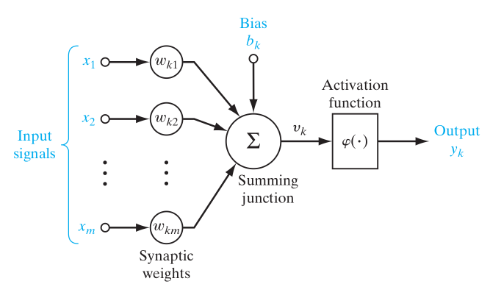
\includegraphics[width=10cm]{Introduction/perceptron-model.png}
\end{figure}
\subsection*{Pattern Recognition}
Neural networks are particularly strong at pattern which in the field is also synonimus of classification. One of the biggest application field for neural networks is computer vision were it is natural to manipulate real numbers which represent intensities in light.\\
The problem of recognizing the ten written digits is extremely complicated for a classic algorithm, where the only sensible approach would be to find some heuristics to classify the inputs. Immediately we would find obstacles to overcome like handling the countless variants in the input.
\subsection*{Ingredients and Terminology}
When first approaching machine learning it can be overwhelming having to learn all the terminology involved. To start we can first list a couple characteristics that can be associated to machine learning models.
\begin{itemize}
    \item Models can be of \textbf{supervised learning} when we are given both the training examples and the labels, or the real answers, the ground truth. They can also be \textbf{unsupervised} when we are not given the labels.
    \item Models can then be \textbf{regression models} when they try to learn a function so that they can predict the expected value in a real space. They can be \textbf{classifiers} and so they identify a set of input as belonging to one of a number of discrete classes. 
\end{itemize}

%%%%%%%%%%%%%%%%%%%%%%%%%%%%%%%%%%%%%%%%%%%%%%%%%%%%%%%%%%%%%%%%%%%
\section{Perceptron}
In our digit classification problem a perceptron would constituite a single computing unit and would be capable of only recognizing one digit. The first elements of the perceptron that we encounter are
\begin{itemize}
    \item a $28 \times 28 = 784$ real vector $\vec{x}$ describing the input or features
    \item an equally sized vector $\vec{w}$ describing the weight associated to every input
    \item a bias "weight" 
\end{itemize}
The last two together are called the parameters of the model and are written as $\Phi$. The perceptron model is governed by a parametric function of x
\[ 
    f_\Phi(x) = \begin{cases}
        1 & if \; b+w\cdot x > 0\\
        0 & otherwise      
    \end{cases} 
\]
\subsection*{Perceptron Algorithm}
If we want to introduce in some way the ground truth, the knowledge that can correct our parameters we can present the perceptron algorithm. It is important to say that, despite having many limitations, if a configuration of the parameters $\Phi$ that makes it so that all training examples are correctly labeled it will find such configuration.
\begin{itemize}
    \item set $b$ and all of the $w$ to 0.
    \item for N iterations, or until the weights do not change
    \begin{itemize}
        \item for each training example $x^k$ with answer $a^k$
        \begin{itemize}
            \item if $a^k-f(x^k) = 0$ continue
            \item else for all weights $w_i, \Delta w_i = (a^k-f(x^k))x_i$
        \end{itemize}
    \end{itemize}
\end{itemize}
It is important to take a look at what the perceptron does, matemathically speaking. It determines the position of the features vector with respect to a plan. It then twiggles that hyperplane with the aim of correctly putting the features vectors that are labeled "yes" above it and those labeled as "no" beneath it.\\
The learning of the model is then represented by the variation of the weights in an effort of correctly identifying all examples.
\subsection*{Terminology}
We have now introduced more elements and we can then take a second to learn the terminology associated with them.
\begin{description}
    \item[Hyperparameters]: these are all "second order" parameters, or more simply, all values that can be changed to impact the performance of the model but that are not the weights or the bias. An example is the number of iterations N.
    \item[Bias]: is a fixed/external knowledge, can be seen as the weight associated with a neuron (feature input) that i always firing, always set to 1.
    \item[Epoch]: an entire run through the training data constituites an epoch.
\end{description}
When multiple computing units share the same inputs we are in multiple classification case and the neural network can be seen as a way to map, in our case, a 784-vector to a 10-vector (each unit deciding whether the input belongs to the i-th class). 